% Priority Application Distribution
% Use with: % Priority Application Distribution
% Use with: % Priority Application Distribution
% Use with: % Priority Application Distribution
% Use with: \input{figures/priority.tex}

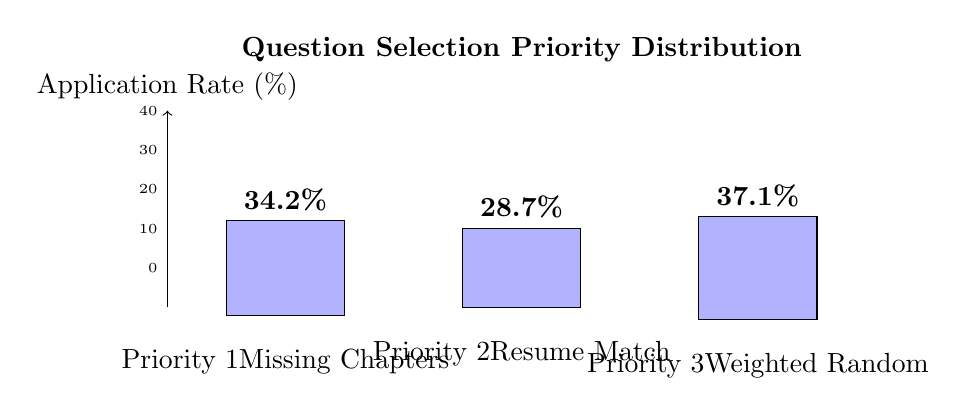
\begin{tikzpicture}[
    bar/.style={rectangle, draw, fill=blue!30, minimum width=1.5cm},
    label/.style={text width=3cm, align=center}
]

% Bars
\node[bar, minimum height=1.2cm] (p1) at (0,0) {};
\node[bar, minimum height=1.0cm] (p2) at (3,0) {};
\node[bar, minimum height=1.3cm] (p3) at (6,0) {};

% Values on bars
\node[above] at (p1.north) {\textbf{34.2\%}};
\node[above] at (p2.north) {\textbf{28.7\%}};
\node[above] at (p3.north) {\textbf{37.1\%}};

% Labels
\node[below=0.3cm] at (p1.south) {Priority 1\\Missing Chapters};
\node[below=0.3cm] at (p2.south) {Priority 2\\Resume Match};
\node[below=0.3cm] at (p3.south) {Priority 3\\Weighted Random};

% Y-axis
\draw[->] (-1.5,-0.5) -- (-1.5,2) node[above] {Application Rate (\%)};
\foreach \y in {0,10,20,30,40}
    \draw (-1.5,\y/20) node[left] {\tiny \y};

% Title
\node[above] at (3,2.5) {\textbf{Question Selection Priority Distribution}};

\end{tikzpicture}



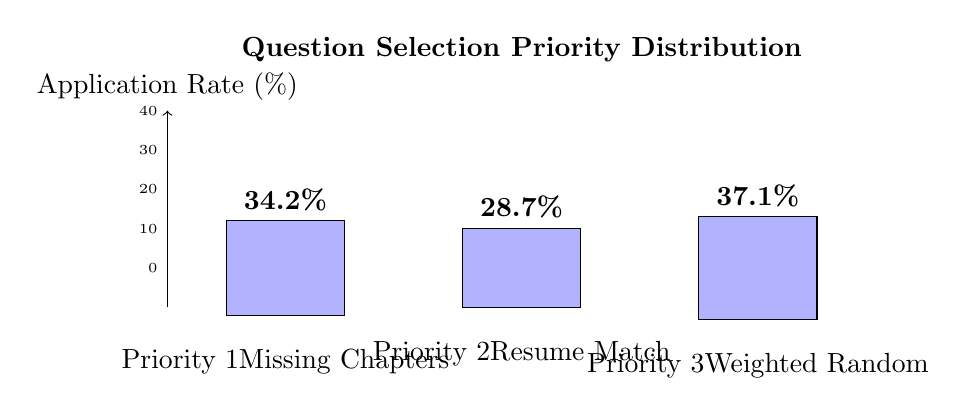
\begin{tikzpicture}[
    bar/.style={rectangle, draw, fill=blue!30, minimum width=1.5cm},
    label/.style={text width=3cm, align=center}
]

% Bars
\node[bar, minimum height=1.2cm] (p1) at (0,0) {};
\node[bar, minimum height=1.0cm] (p2) at (3,0) {};
\node[bar, minimum height=1.3cm] (p3) at (6,0) {};

% Values on bars
\node[above] at (p1.north) {\textbf{34.2\%}};
\node[above] at (p2.north) {\textbf{28.7\%}};
\node[above] at (p3.north) {\textbf{37.1\%}};

% Labels
\node[below=0.3cm] at (p1.south) {Priority 1\\Missing Chapters};
\node[below=0.3cm] at (p2.south) {Priority 2\\Resume Match};
\node[below=0.3cm] at (p3.south) {Priority 3\\Weighted Random};

% Y-axis
\draw[->] (-1.5,-0.5) -- (-1.5,2) node[above] {Application Rate (\%)};
\foreach \y in {0,10,20,30,40}
    \draw (-1.5,\y/20) node[left] {\tiny \y};

% Title
\node[above] at (3,2.5) {\textbf{Question Selection Priority Distribution}};

\end{tikzpicture}



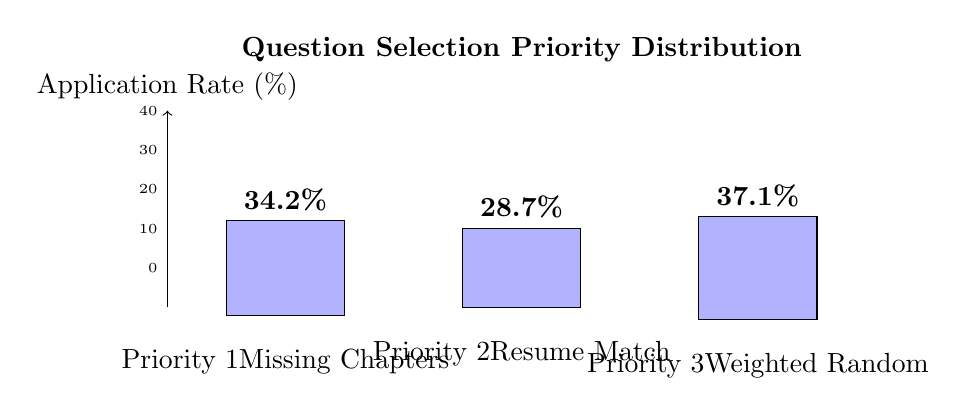
\begin{tikzpicture}[
    bar/.style={rectangle, draw, fill=blue!30, minimum width=1.5cm},
    label/.style={text width=3cm, align=center}
]

% Bars
\node[bar, minimum height=1.2cm] (p1) at (0,0) {};
\node[bar, minimum height=1.0cm] (p2) at (3,0) {};
\node[bar, minimum height=1.3cm] (p3) at (6,0) {};

% Values on bars
\node[above] at (p1.north) {\textbf{34.2\%}};
\node[above] at (p2.north) {\textbf{28.7\%}};
\node[above] at (p3.north) {\textbf{37.1\%}};

% Labels
\node[below=0.3cm] at (p1.south) {Priority 1\\Missing Chapters};
\node[below=0.3cm] at (p2.south) {Priority 2\\Resume Match};
\node[below=0.3cm] at (p3.south) {Priority 3\\Weighted Random};

% Y-axis
\draw[->] (-1.5,-0.5) -- (-1.5,2) node[above] {Application Rate (\%)};
\foreach \y in {0,10,20,30,40}
    \draw (-1.5,\y/20) node[left] {\tiny \y};

% Title
\node[above] at (3,2.5) {\textbf{Question Selection Priority Distribution}};

\end{tikzpicture}



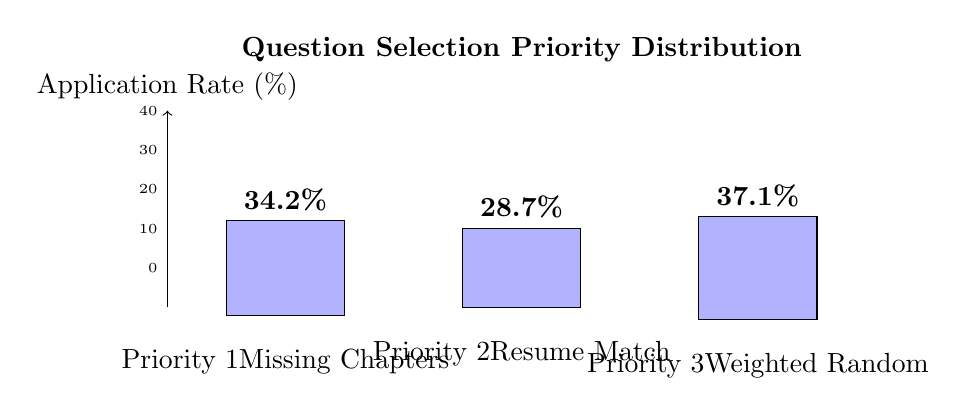
\begin{tikzpicture}[
    bar/.style={rectangle, draw, fill=blue!30, minimum width=1.5cm},
    label/.style={text width=3cm, align=center}
]

% Bars
\node[bar, minimum height=1.2cm] (p1) at (0,0) {};
\node[bar, minimum height=1.0cm] (p2) at (3,0) {};
\node[bar, minimum height=1.3cm] (p3) at (6,0) {};

% Values on bars
\node[above] at (p1.north) {\textbf{34.2\%}};
\node[above] at (p2.north) {\textbf{28.7\%}};
\node[above] at (p3.north) {\textbf{37.1\%}};

% Labels
\node[below=0.3cm] at (p1.south) {Priority 1\\Missing Chapters};
\node[below=0.3cm] at (p2.south) {Priority 2\\Resume Match};
\node[below=0.3cm] at (p3.south) {Priority 3\\Weighted Random};

% Y-axis
\draw[->] (-1.5,-0.5) -- (-1.5,2) node[above] {Application Rate (\%)};
\foreach \y in {0,10,20,30,40}
    \draw (-1.5,\y/20) node[left] {\tiny \y};

% Title
\node[above] at (3,2.5) {\textbf{Question Selection Priority Distribution}};

\end{tikzpicture}

